%% abtex2-modelo-slides.tex, v-1.0 gfabinhomat
%% Copyright 2012-2018 by abnTeX2 group at http://www.abntex.net.br/ 
%%
%% This work may be distributed and/or modified under the
%% conditions of the LaTeX Project Public License, either version 1.3
%% of this license or (at your option) any later version.
%% The latest version of this license is in
%%   http://www.latex-project.org/lppl.txt
%% and version 1.3 or later is part of all distributions of LaTeX
%% version 2005/12/01 or later.
%%
%% This work has the LPPL maintenance status `maintained'.
%% 
%% The Current Maintainer of this work is Fábio Rodrigues Silva, 
%% member of abnTeX2 team, led by Lauro César Araujo. 
%% Further information are available on 
%% http://www.abntex.net.br/
%%
%% This work consists of the files abntex2-modelo-slides.tex, 
%% abntex2-modelo-references.bib and abntex2-modelo-marca.pdf
%%
%% Modelo desenvolvido por Fábio Rodrigues Silva (gfabinhomat@gmail.com)
%% Mais informações podem ser obtidas no guia do usuário Beamer 
%% (http://linorg.usp.br/CTAN/macros/latex/contrib/beamer/doc/beameruserguide.pdf)
%% Informações rápidas podem ser acessadas em http://en.wikibooks.org/wiki/LaTeX/Presentations


% Apresentações em widescreen. Outros valores possíveis: 1610, 149, 54, 43 e 32.
% Por padrão, as apresentações são no formato 4:3 (sem o aspectratio).
\documentclass[aspectratio=169]{beamer}	 	

\usetheme{Pittsburgh}
\usecolortheme{default}
\usefonttheme[onlymath]{serif}			% para fontes matemáticas
% Enconte mais temas e cores em http://www.hartwork.org/beamer-theme-matrix/ 
% Veja também http://deic.uab.es/~iblanes/beamer_gallery/index.html

% Customizações de Cores: fg significa cor do texto e bg é cor do fundo

\setbeamercolor{author}{fg=black}
\setbeamercolor{institute}{fg=black}
\setbeamercolor{date}{fg=black}
\setbeamercolor{frametitle}{fg=black}

% ---
% PACOTES
% ---
\usepackage[alf]{abntex2cite}		% Citações padrão ABNT
\usepackage[brazil]{babel}		% Idioma do documento
\usepackage{color}			% Controle das cores
\usepackage[T1]{fontenc}		% Selecao de codigos de fonte.
\usepackage{graphicx}			% Inclusão de gráficos
\usepackage[utf8]{inputenc}		% Codificacao do documento (conversão automática dos acentos)
\usepackage{txfonts}			% Fontes virtuais
% ---
\usepackage{tcolorbox}
\usepackage{ragged2e}
\usepackage{tikz}
\usetikzlibrary{arrows.meta, positioning, shapes.geometric}
\usepackage{soul}

% --- Informações do documento ---
\title{Tensor Processing Units (TPUs)}

\author{
Eduardo Rabelo Feitosa \\
\and
Joao Paulo Lopes}


\institute{Universidade Federal do Vale do São Francisco
	    \par
	    CECOMP}
\date{\today, v-1.9.7}
% ---

% ----------------- INÍCIO DO DOCUMENTO --------------------------------------
\begin{document}

% ----------------- SLIDE 1: TÍTULO -----------------
\begin{frame}
\begin{minipage}{1\linewidth}
  \centering
  \begin{tabular}{cc}
    \begin{tabular}{c}
      
\includegraphics[width=3.5cm]{images/Marca Univasf Completa (Sem fundo).png}
    \end{tabular}
    &
    \begin{tabular}{c}
      \textbf{Universidade Federal do Vale do São Francisco} \\ \textbf{CECOMP}
    \end{tabular}
  \end{tabular}
\end{minipage}
\titlepage
\end{frame}

% ----------------- SLIDE 2: SUMÁRIO -----------------
\begin{frame}{Sumário}
\tableofcontents
\end{frame}

% ===== SEÇÃO 1: FUNDAMENTAÇÃO =====
\section{Fundamentação}

% ----------------- SLIDE 3: CONTEXTO E MOTIVAÇÃO -----------------
\begin{frame}{Contexto e Motivação}

\begin{columns}

\column{0.5\textwidth}
\justify
\small{
"Starting as early as 2006, we discussed deploying GPUs, FPGAs, or \textbf{custom ASICs} in our datacenters. We concluded that the
few applications that could run on special hardware could be done virtually [...] The conversation changed in 2013 when a projection where people use\textbf{ voice search} for 3 minutes a day using speech recognition DNNs\textbf{ would require our datacenters to double to meet }\textbf{computation demands}, which would be very expensive to satisfy with conventional CPUs. Thus, we started a high-priority project to
quickly produce \textbf{a custom ASIC for inference} [...]''\\ }

\column{0.5\textwidth}

\centering
\begin{tikzpicture}
\node[inner sep=0] (img) {
  \fbox{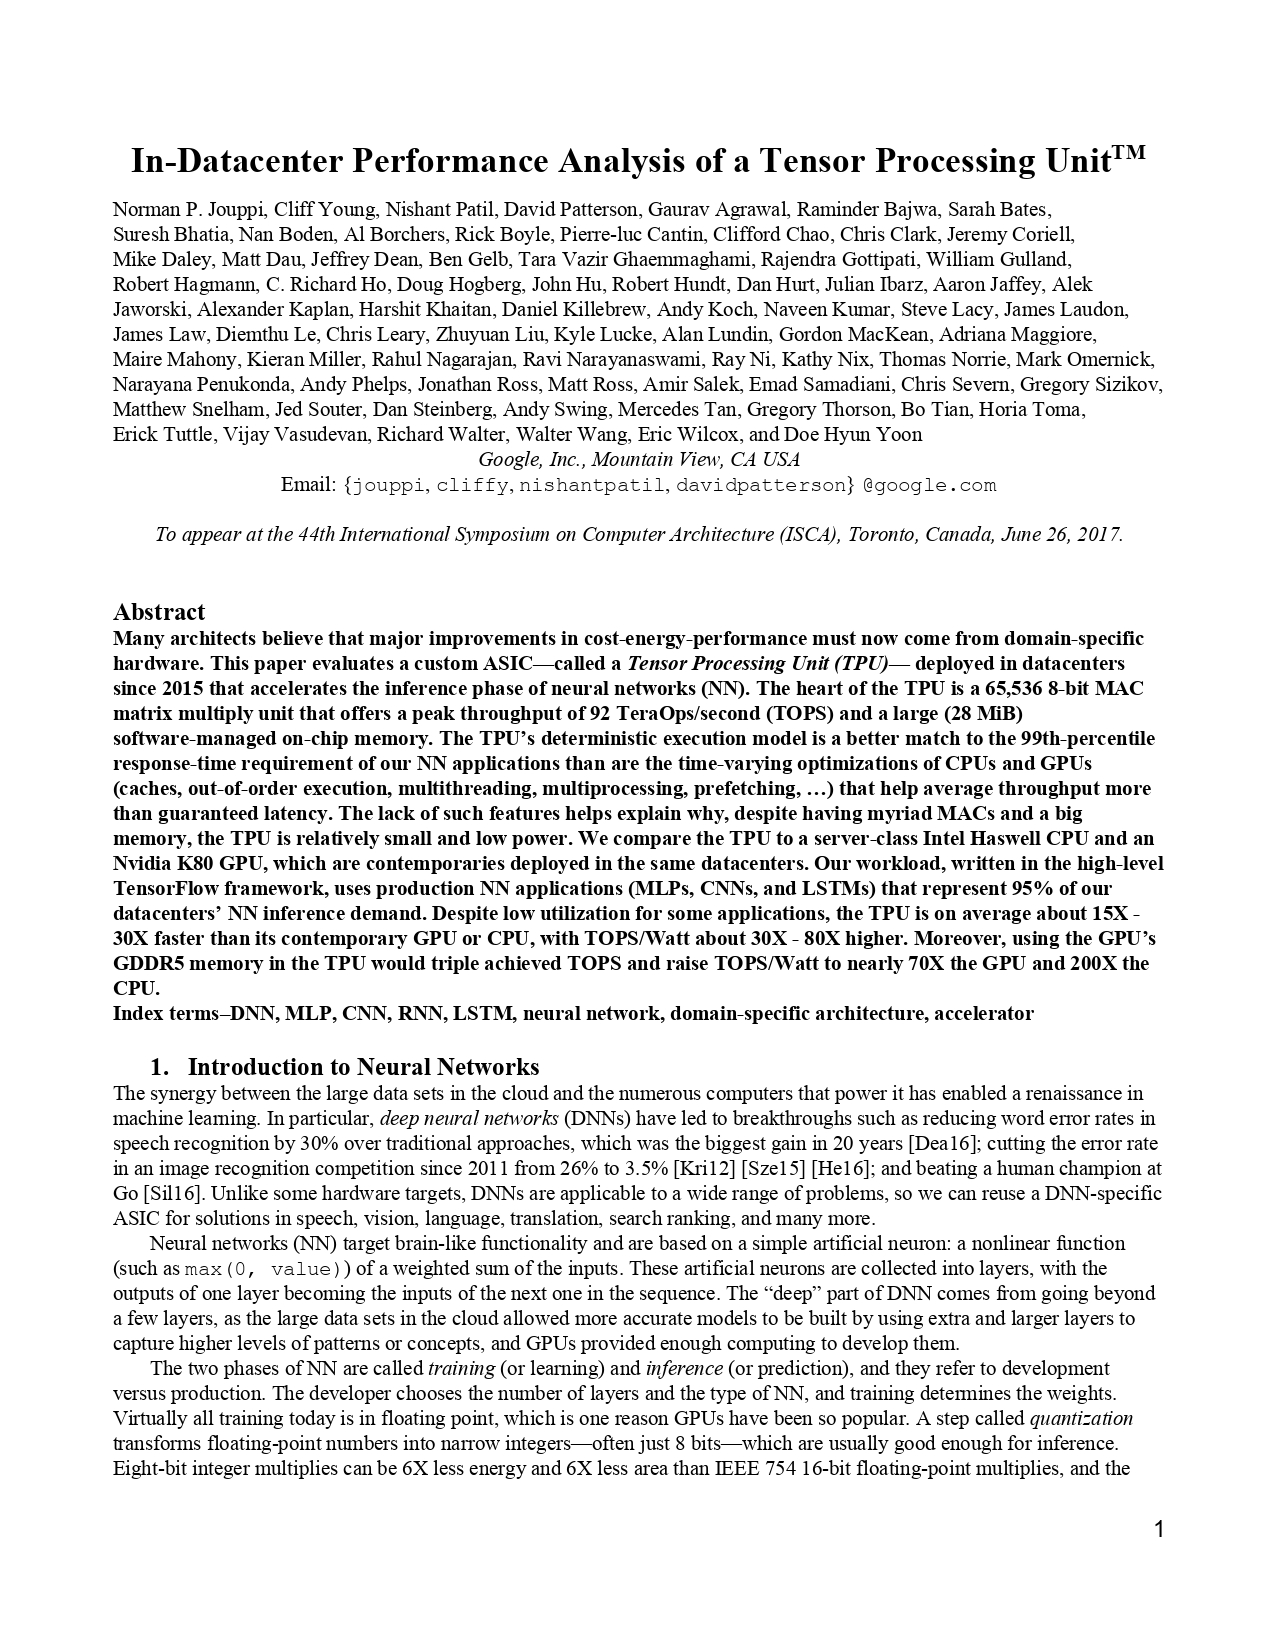
\includegraphics[
    width=2.5\linewidth,
    height=6cm,
    keepaspectratio,
    trim=0 250 0 0,
    clip
  ]{images/tpu_paper_first_page_page-0001.jpg}}
};


\node[
  anchor=south east,
  fill=black!70,
  text=white,
  font=\scriptsize,
  inner sep=2pt
] at (img.south east) {\cite{jouppi2017tpu}};


\end{tikzpicture}

\end{columns}

\end{frame}

% ===== SEÇÃO 2: TENSORES =====
%\section{Tensores}

% ----------------- SLIDE 3: O QUE SÃO TENSORES? -----------------
\begin{frame}{O que são Tensores?}

\begin{columns}

\column{0.55\textwidth}
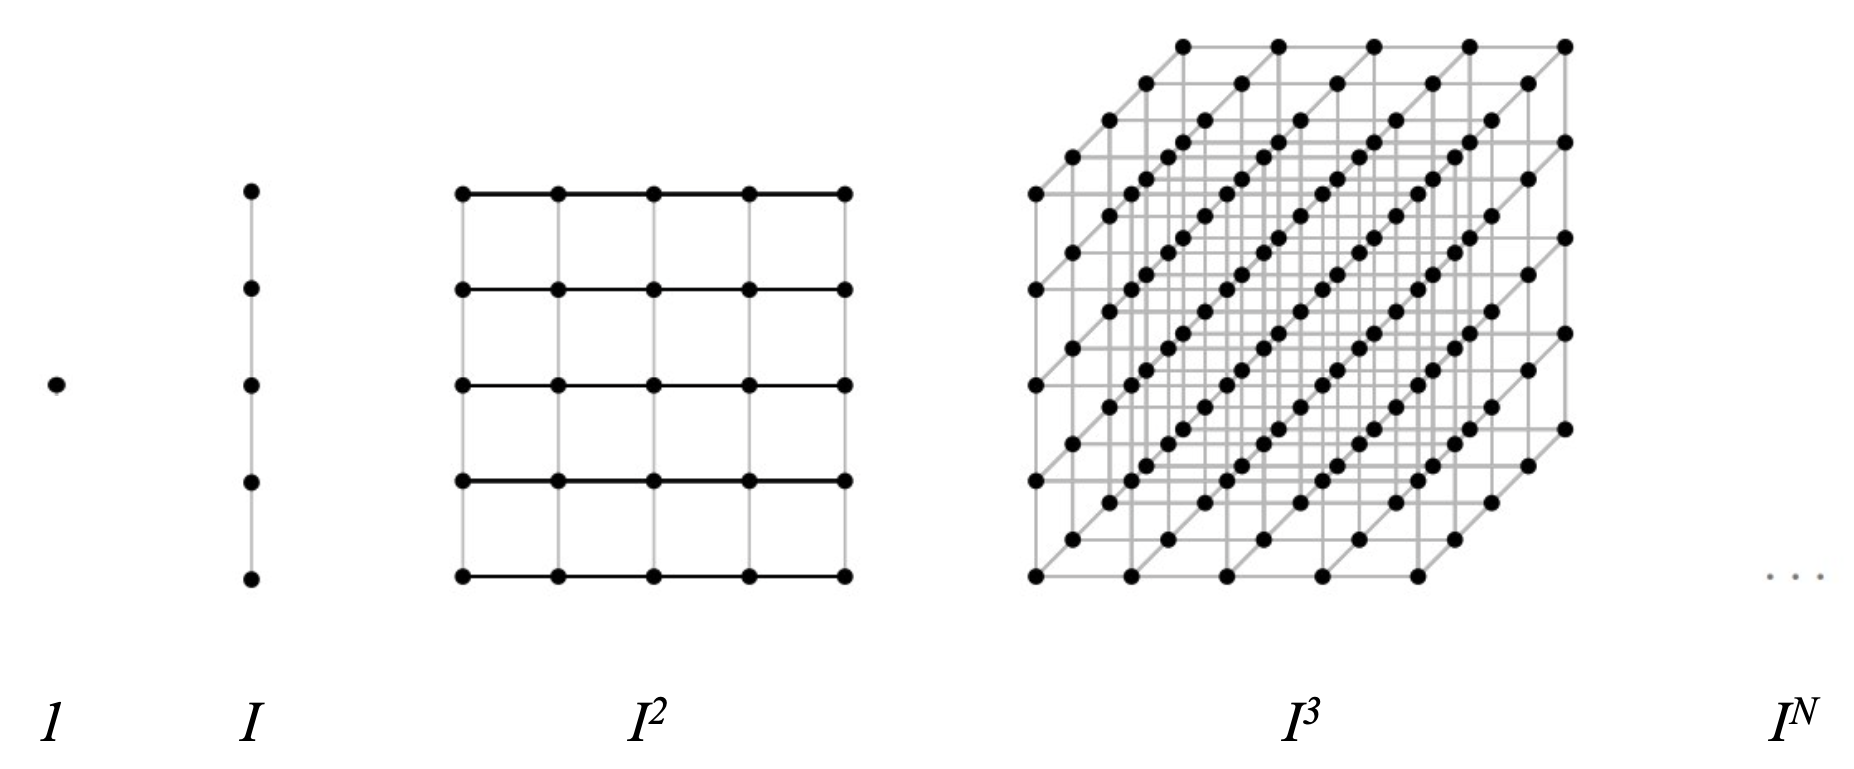
\includegraphics[width=\textwidth]{images/tensor_example.png}

\column{0.45\textwidth}

Tensores generalizam arrays para N dimensões:
\begin{itemize}

\item \textbf{Escalar} (rank 0): um valor — ex: temperatura 
\item \textbf{Vetor} (rank 1): array 1D — ex: lista 
\item \textbf{Matriz} (rank 2): array 2D — ex: matriz 
\item \textbf{Tensor} (rank $\geq$ 3): ex: imagem RGB $(H \times W \times 3)$
\end{itemize}

\end{columns}

\end{frame}

% ===== SEÇÃO 3: MICROARQUITETURA =====
\section{Microarquitetura}

% ----------------- SLIDE 5: VISÃO GERAL DA MICROARQUITETURA -----------------
\begin{frame}{Visão Geral da Microarquitetura}
  % Inserir Figura 1 do paper (block diagram)
  \begin{columns}
    \column{0.55\textwidth}
      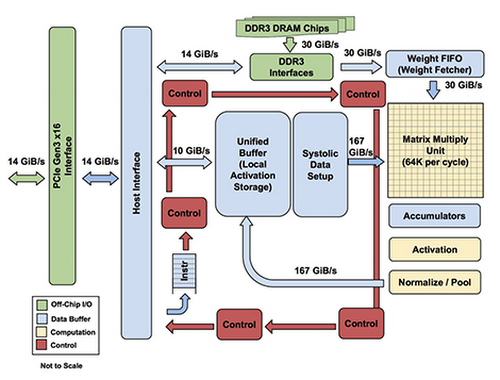
\includegraphics[width=\textwidth]{images/tpu_block_diagram2.png} % substituir pelo arquivo real
    \column{0.45\textwidth}
      \textbf{Componentes principais}
      \begin{itemize}
        \item{ \justify Conectado ao host via \textbf{PCIe Gen3 x16}}
        \item{ \justify \textbf{Matrix Multiply Unit (MXU)}: 256×256 MACs de 8 bits = 65.536 operações/ciclo}
        \item{ \justify \textbf{Unified Buffer (UB)}: 24 MiB on-chip para ativações}
        \item{ \justify \textbf{Accumulators}: 4 MiB de acumuladores de 32 bits}
        \item{ \justify \textbf{Weight FIFO}: carrega pesos da Weight Memory (8 GiB DRAM off-chip)}
        \item{ \justify \textbf{Activation Unit}: aplica funções não-lineares (ReLU, Sigmoid)}
        
      \end{itemize}
  \end{columns}
  \vfill
 
\end{frame}

% ----------------- SLIDE 6: SYSTOLIC ARRAY -----------------
\begin{frame}{Systolic Array: o coração da TPU}
  \begin{columns}
    \column{0.5\textwidth}
      % Inserir Figura 4 do paper (systolic data flow)
      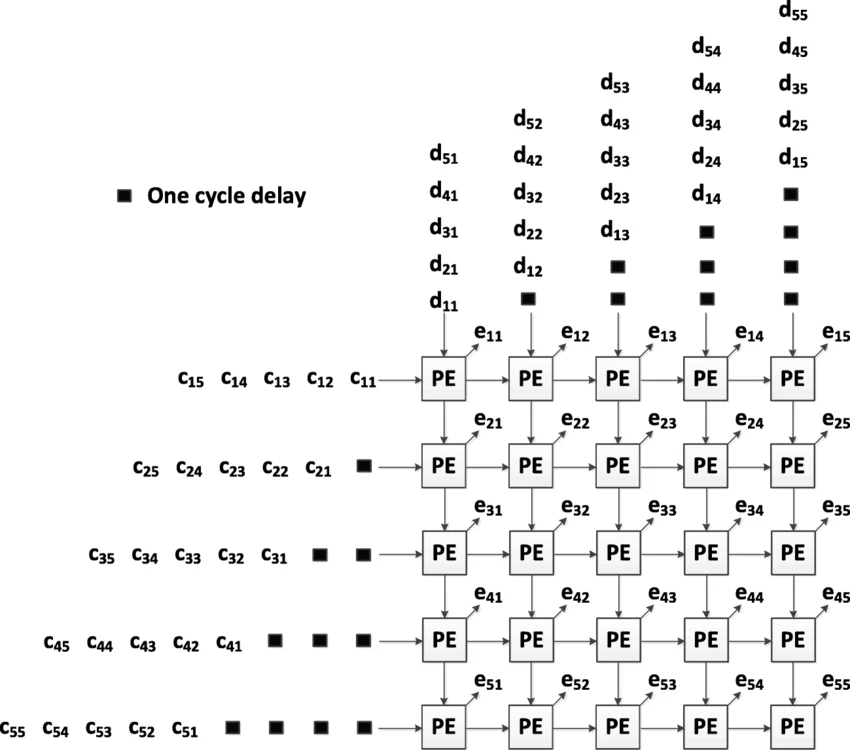
\includegraphics[width=\textwidth]{images/tpu_systolic.png} % substituir pelo arquivo real
    \column{0.5\textwidth}
      \textbf{Como funciona}
      
      \begin{itemize}
        \item {\justify Dados de entrada fluem da \textbf{esquerda}}
        \item {\justify Pesos são pré-carregados pelo \textbf{topo}}
        \item {\justify Cada célula multiplica e acumula, passando o resultado para a próxima}
        \item {\justify Uma operação de 256 elementos percorre a matriz como \textbf{onda diagonal}} \cite{kung1980systolic}
      \end{itemize}
      \small
      \justify
      "\textbf{Software has the illusion that each 256B input is read at once}, and they instantly update one location of each of 256 accumulator RAMs'' \cite{jouppi2017tpu}.
    
  \end{columns}
\end{frame}

% ----------------- SLIDE 7: PIPELINE E MODELO DE EXECUÇÃO -----------------
\begin{frame}{Pipeline e Modelo de Execução}
  \begin{columns}
    \column{0.5\textwidth}
\justify{
\small
\emph{"\textbf{We don’t have clean pipeline overlap diagrams}, because our CISC instructions can occupy a station for\textbf{ thousands of clock cycles}, unlike the traditional RISC pipeline with one clock cycle per stage." \cite{jouppi2017tpu}}
} \\[0.5cm]
    \vfill
    
      \textbf{ISA CISC}
      \begin{itemize}
        \item{\justify 12 instruções no total; CPI de 10 a 20 ciclos}
        \item{\justify  Instruções enviadas pelo host CPU via PCIe}
        \item{\justify Pipeline de \textbf{4 estágios}, um por instrução ((1) Fetch/Decode, (2) Memory Read, (3) Execute, (4) Memory Write)}
        
      \end{itemize}
     
    \column{0.5\textwidth}
      \textbf{Modelo determinístico}
      \\[0.5cm]
      \begin{itemize}
      
        \item{\justify \textbf{Single-threaded}: sem multithreading, sem context switching}\\[.5cm]
        \item{\justify \textbf{Sem caches}: sem cache miss, sem especulação}\\[.5cm]
        \item{\justify Execução \textbf{previsível e repetível}: ideal para requisitos de latência no percentil 99}\\[.5cm]
        \item{\justify Instruções ocupam \textbf{milhares de ciclos} por estágio}
      \end{itemize}
      \vfill
  \end{columns}
\end{frame}

% ----------------- SLIDE 8: PRINCIPAIS INTRUÇÕES DA TPU -----------------

\begin{frame}{Principais Instruções da TPU}
\centering

\begin{tikzpicture}[
  node distance=1.8cm,
  every node/.style={font=\scriptsize},
  box/.style={
    rectangle, rounded corners=3pt,
    minimum width=2.4cm, minimum height=0.85cm,
    align=center, draw, thick
  },
  gbox/.style={box, fill=gray!15,   draw=gray!50},
  tbox/.style={box, fill=teal!15,   draw=teal!50},
  pbox/.style={box, fill=violet!15, draw=violet!50},
  abox/.style={box, fill=orange!15, draw=orange!40},
  rbox/.style={box, fill=red!12,    draw=red!40},
  arr/.style={->, >=stealth, thick, shorten >=2pt, shorten <=2pt},
  lbl/.style={font=\tiny, fill=white, inner sep=1.5pt}
]

% left column (host side)
\node[gbox] (cpu)   at (-3,  -1)  {\textbf{CPU host}\\[-1pt]{\tiny host memory}};
\node[gbox] (wmem)  at (-3, -3)  {\textbf{Weight Memory}\\[-1pt]{\tiny 8\,GiB DRAM}};

% center column (on-chip memory)
\node[tbox] (ub)    at (2,  -1)  {\textbf{Unified Buffer}\\[-1pt]{\tiny 24\,MiB}};
\node[gbox] (wfifo) at (2, -3)  {\textbf{Weight FIFO}\\[-1pt]{\tiny tiles}};

% right column (compute core)
\node[pbox] (mxu)   at (7, -1) {\textbf{Matrix Unit}\\[-1pt]{\tiny 256$\times$256 MACs}};

% vertical compute stack (centered around MXU)
\node[abox] (acc)   at (7,  1) {\textbf{Accumulators}\\[-1pt]{\tiny 32-bit}};
\node[rbox] (act)   at (2,  1) {\textbf{Activation}\\[-1pt]{\tiny ReLU, Sigmoid}};

% ======================
% FLOWS
% ======================

% host <-> UB
%\draw[arr] (cpu.east)
%  -- node[lbl, above]{\textbf{(2) Read}} (ub.west);

\draw[arr] (cpu.east)
  -- node[lbl, above=5pt]{\textbf{(2) Read\_Host\_Memory}} (ub.west);

\draw[arr] (ub.west)
  -- node[lbl, below=5pt]{\textbf{(4) Write\_Host\_Memory}} (cpu.east);

% weights path
\draw[arr] (wmem.east)
  -- node[lbl, below=5pt]{\textbf{(2) Read\_Weights}} (wfifo.west);

% FIFO -> MXU
\draw[arr] (wfifo.east)
  -- (mxu.south);

% UB -> MXU
\draw[arr] (ub.east)
  -- node[lbl, above]{\textbf{(3) MatrixMultiply}} (mxu.west);

% MXU -> Acc
\draw[arr] (mxu.north)
  -- (acc.south);

% Acc -> Activation (re-centered)
\draw[arr] (acc.west)
  -- node[lbl, above]{\textbf{(3) Activate}} (act.east);

% Activation -> UB (feedback loop)
\draw[arr] (act.south)
  -- (ub.north);

% PCIe incoming arrow
\draw[arr, dashed] (-3, 0.5) -- (cpu.north)
  node[pos=0.15, above, xshift=-0mm, font=\tiny]{(1) PCIe Gen3 x16};

\end{tikzpicture}
\end{frame}

% ===== SEÇÃO 9: COMPARAÇÃO ARQUITETURAL =====
\section{Comparação Arquitetural}

% ----------------- SLIDE 

\begin{frame}{TPU vs RISC/CISC}
\centering
\vspace{0.3cm}

\begin{columns}

\column{0.46\textwidth}
\begin{tcolorbox}[colback=blue!5, colframe=blue!40, title=\centering\textbf{CPU moderna}]
\begin{itemize}
  \item Cache hierárquico (L1/L2/L3)
  \item Branch prediction
  \item Execução fora de ordem
  \item Multithreading
  \item ISA de propósito geral
\end{itemize}
\vspace{0.2cm}
\centering\footnotesize $\to \quad$Projetada para \textbf{qualquer} workload
\end{tcolorbox}

\column{0.08\textwidth}
\centering
{\Huge \textbf{vs}}

\column{0.46\textwidth}
\begin{tcolorbox}[colback=red!5, colframe=red!40, title=\centering\textbf{TPU v1}]
\begin{itemize}
  \item Sem cache
  \item Sem branch prediction
  \item in-order
  \item single-thread
  \item Apenas 12 instruções matriciais
\end{itemize}
\vspace{0.2cm}
\centering\footnotesize $\to \quad $Projetada para \textbf{uma} operação
\end{tcolorbox}

\end{columns}

\vfill

\end{frame}
\begin{frame}{Comparação Visual}
        \begin{figure}
            \centering
            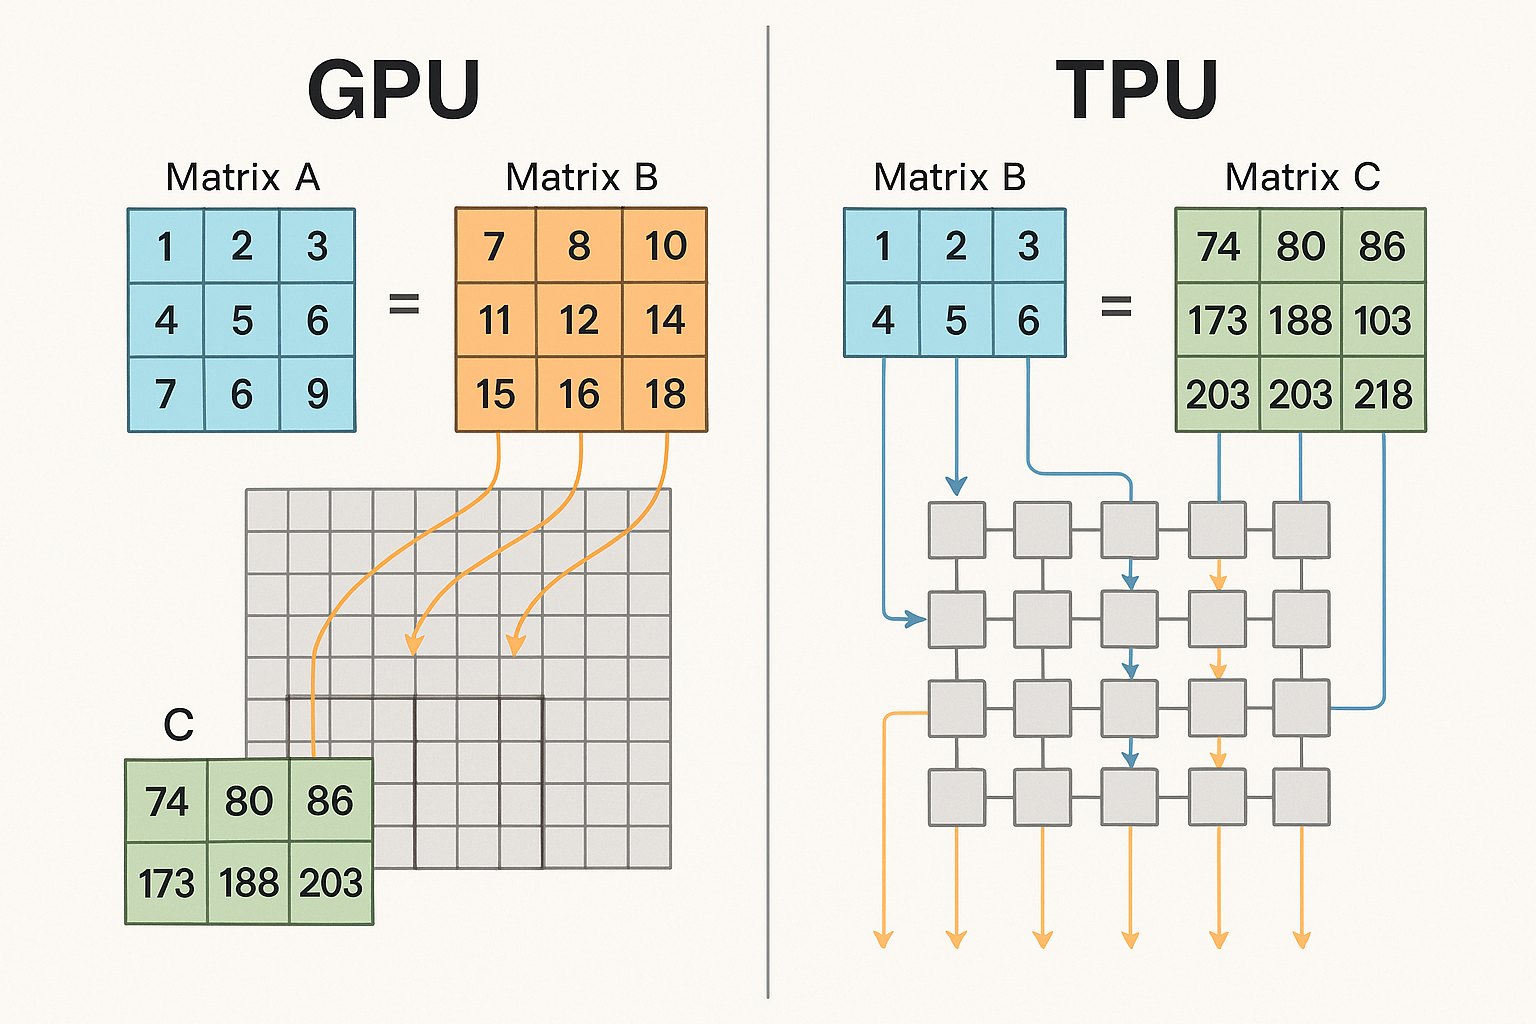
\includegraphics[width=0.8\linewidth]{images/GPUvsTPU-1.png}
        \end{figure}
\end{frame}
%===== SEÇÃO 6: =====
\section{Análise Crítica}

\begin{frame}{Desempenho: Modelo Roofline}
\begin{columns}
  \column{0.58\textwidth}
  \centering{
    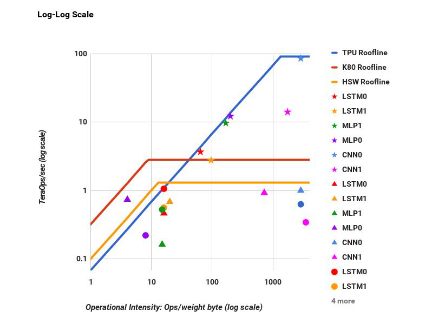
\includegraphics[width=\textwidth]{images/tpu_roofline.png}
    Ops/weight byte $\times$ TeraOps/sec
    }
  \column{0.42\textwidth}

   \justify{
     O modelo Roofline relaciona num gráfico 2D: \textbf{desempenho de ponto flutuante, intensidade operacional e desempenho de memória.}
      \hfill\cite{williams2009roofline}
}
   \\[0.5cm]
   
    TPU opera \textbf{15×--30×} mais rápido que CPU e GPU contemporâneas\\[0.4cm]
    Com limite de latência de 7ms (p99):\\[-0.1cm]
    \begin{itemize}
      \item CPU: 42\% da capacidade
      \item GPU: 37\% da capacidade
      \item TPU: \textbf{80\%} da capacidade
    \end{itemize}
    
\end{columns}
\end{frame}

\begin{frame}{Eficiência e Escala}
\begin{columns}
  \column{0.5\textwidth}
    \textbf{Eficiência energética}\\[0.3cm]
    \vfill
    \centering{
    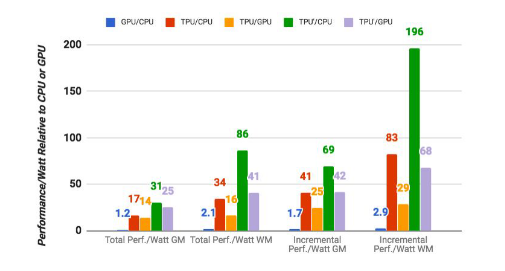
\includegraphics[width=8.4cm]{images/tpu_perf_watt.png}\\[0.2cm]
    Performance/Watt em relação a CPU ou GPU
}
  \column{0.5\textwidth}
    \textbf{Evolução de escala}\\[0.3cm]
    \begin{tabular}{lrr}
\hline
\textbf{Geração} & \textbf{Chips/Pod} & \textbf{Escala}\\
\hline
TPU v1 & 1      & — \\
TPU v2 & 256    & 256× \\
TPU v3 & 1.024  & 4× \\
TPU v4 & 4.096  & 4× \\
TPU v7 & 9.216  & 2,25× \\
\hline
\end{tabular}
    \vspace{0.4cm}
    \justify
    O Ironwood (TPU v7) foi projetado explicitamente para a era da \textbf{inferência em larga escala}, entregando 2× mais performance/watt que a geração anterior. Modelos como Gemini e Claude hoje treinam inteiramente sobre TPUs
    
\end{columns}
\end{frame}

\begin{frame}{Limitações}

\begin{itemize}
  \item {\justify \textbf{Memory-bound:} cargas de trabalho reais são limitadas pela largura de banda de memória, não pela capacidade de cálculos. MACs ficam ociosos esperando dados
  \cite{jouppi2017tpu}}
  
  \item {\justify \textbf{Fragmentação interna da MXU:}
  aumentar a matrix unit de 256$\times$256 para
  512$\times$512 \textit{piora} o desempenho médio. 
  Matrizes menores desperdiçam MACs em duas dimensões}

  \item { \justify \textbf{Baixa proporcionalidade energética:}
  a 10\% de carga, a TPU consome 88\% da potência
  máxima}

  \item{\justify \textbf{Só faz uma coisa:}
  Extremamente eficiente para multiplicação de matrizes densas, mas inútil para qualquer outra tarefa: a TPU não busca instruções, não gerencia memória, não tem sistema operacional. É um coprocessador que depende inteiramente da CPU host para funcionar}
\end{itemize}

\end{frame}

\section{Aplicações}
\begin{frame}{Aplicações}

\centering

\begin{columns}[c] % alinhamento vertical consistente

\column{0.5\textwidth}
\centering
% GEMINI
\begin{tikzpicture}
\node[inner sep=0] (img) {
  \fbox{
\includegraphics[
    width=0.9\linewidth,
    height=3.5cm,
    keepaspectratio,
    trim=120 0 120 0,
    clip
  ]{images/gemini.png}}
};

\node[
  anchor=north west,
  fill=black!70,
  text=white,
  font=\scriptsize,
  inner sep=2pt
] at (img.north west) {Gemini};


\node[
  anchor=south east,
  fill=black!70,
  text=white,
  font=\scriptsize,
  inner sep=2pt
] at (img.south east) {\cite{gemini2025}};


\end{tikzpicture}

\vspace{0.4cm}
% ALPHAFOLD
\begin{tikzpicture}
\node[inner sep=0] (img) {
  \fbox{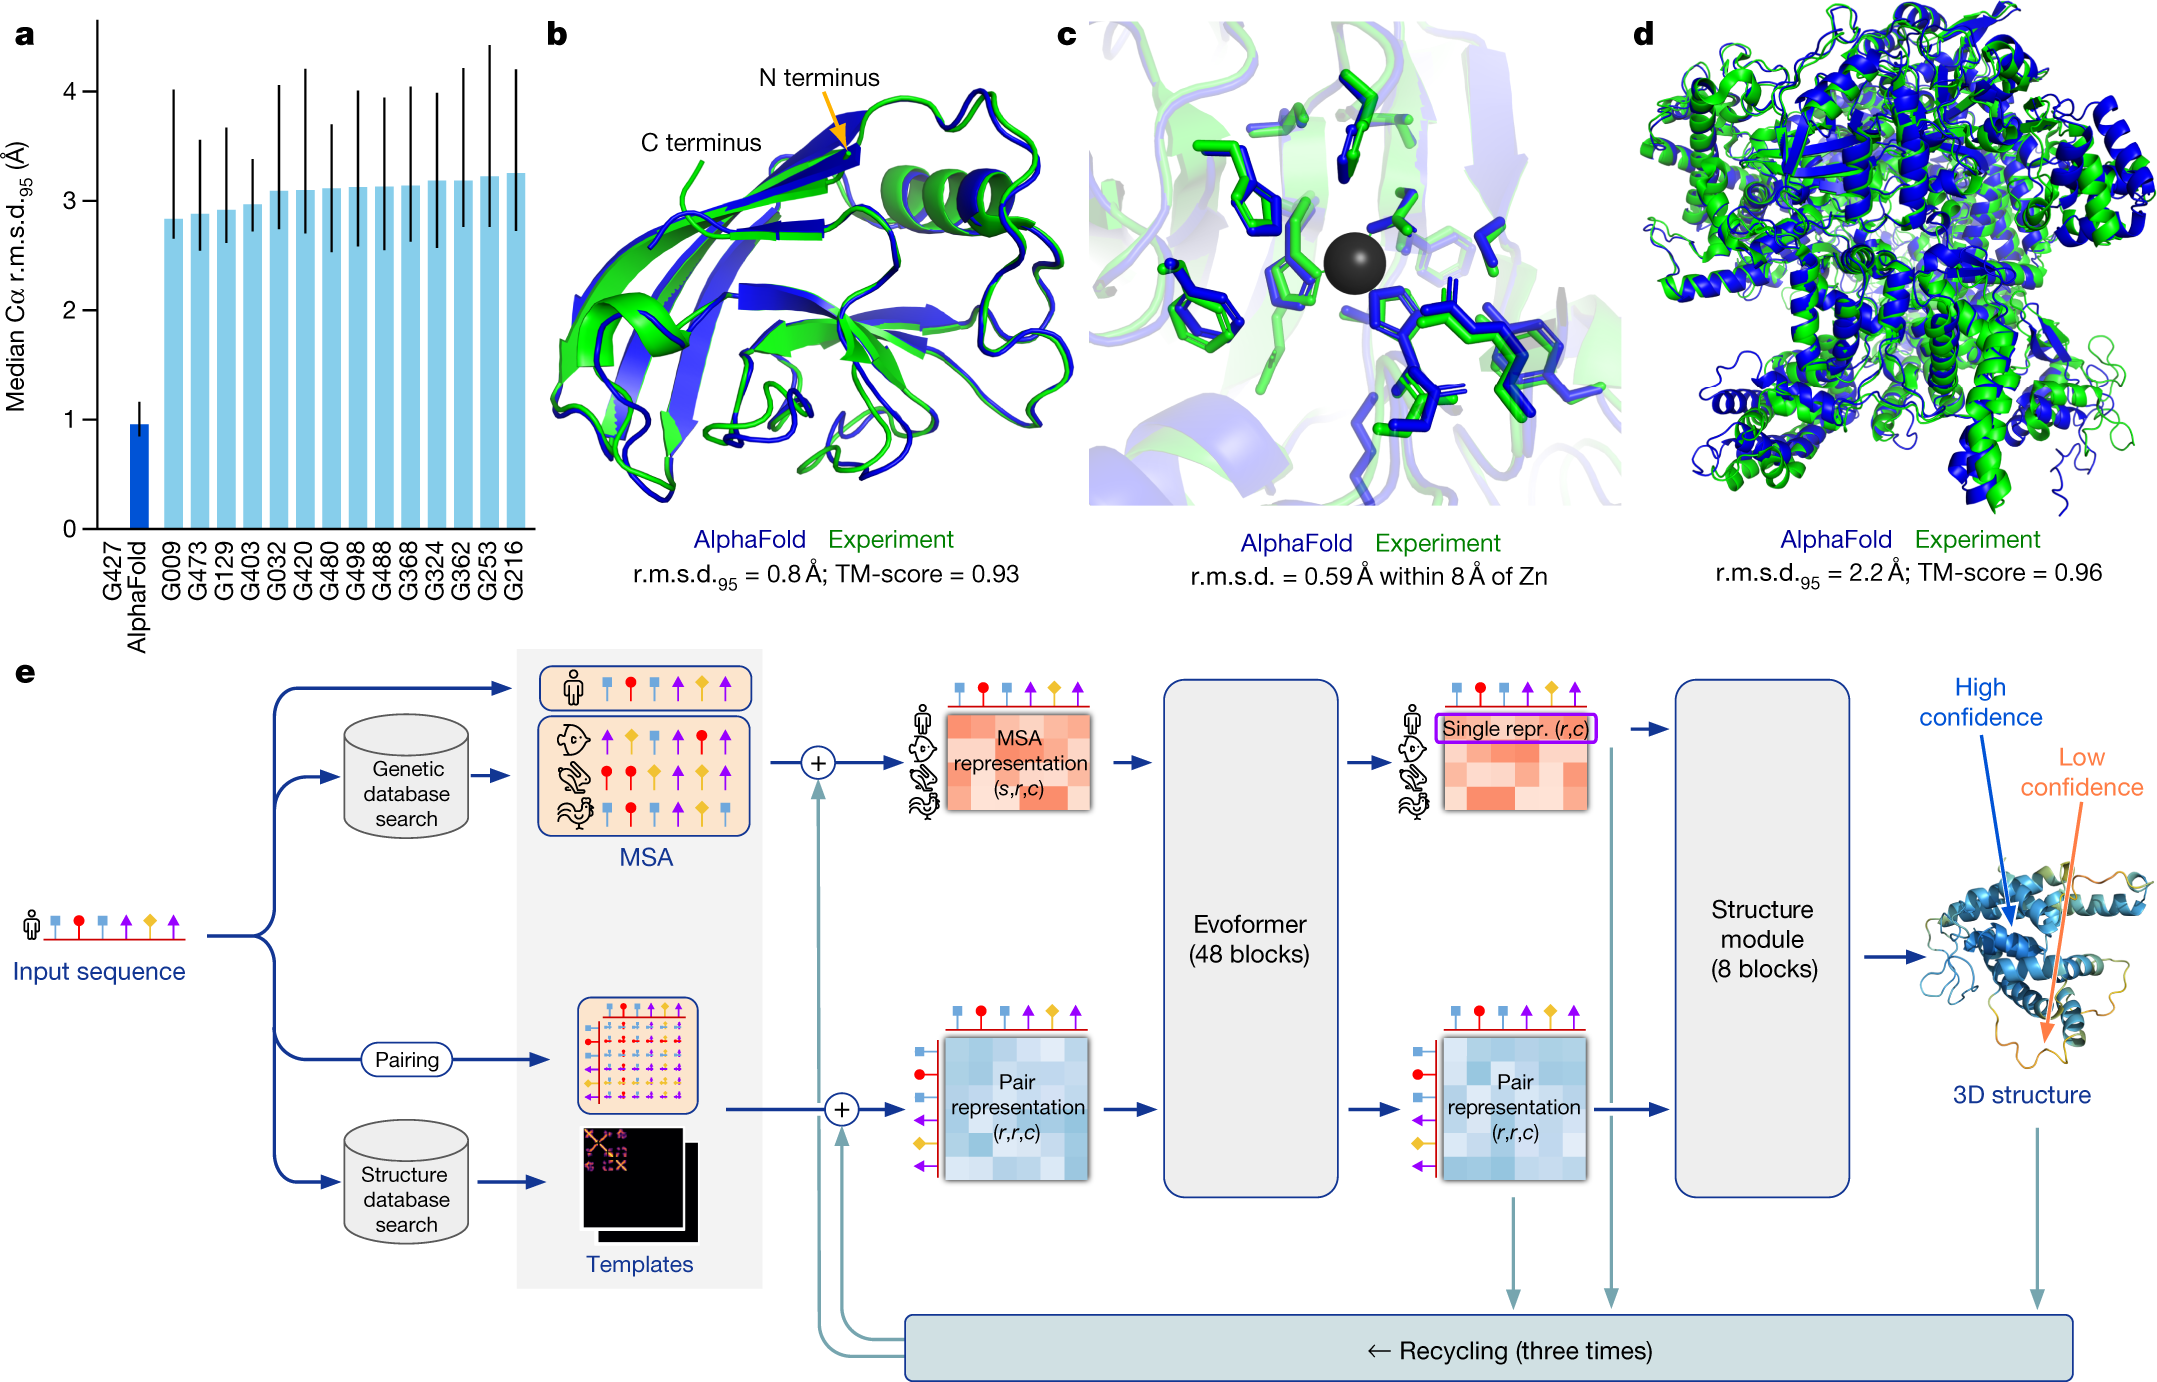
\includegraphics[
    width=0.9\linewidth,
    height=3.5cm,
    keepaspectratio
  ]{images/alphafold2.png}}
};

\node[
  anchor=north west,
  fill=black!70,
  text=white,
  font=\scriptsize,
  inner sep=2pt
] at (img.north west) {AlphaFold 2};

\node[
  anchor=south east,
  fill=black!70,
  text=white,
  font=\scriptsize,
  inner sep=2pt
] at (img.south east) {\cite{jumper2021alphafold}};


\end{tikzpicture}


\column{0.5\textwidth}
\centering

% TPU-GEN

\begin{tikzpicture}
\node[inner sep=0] (img) {
  \fbox{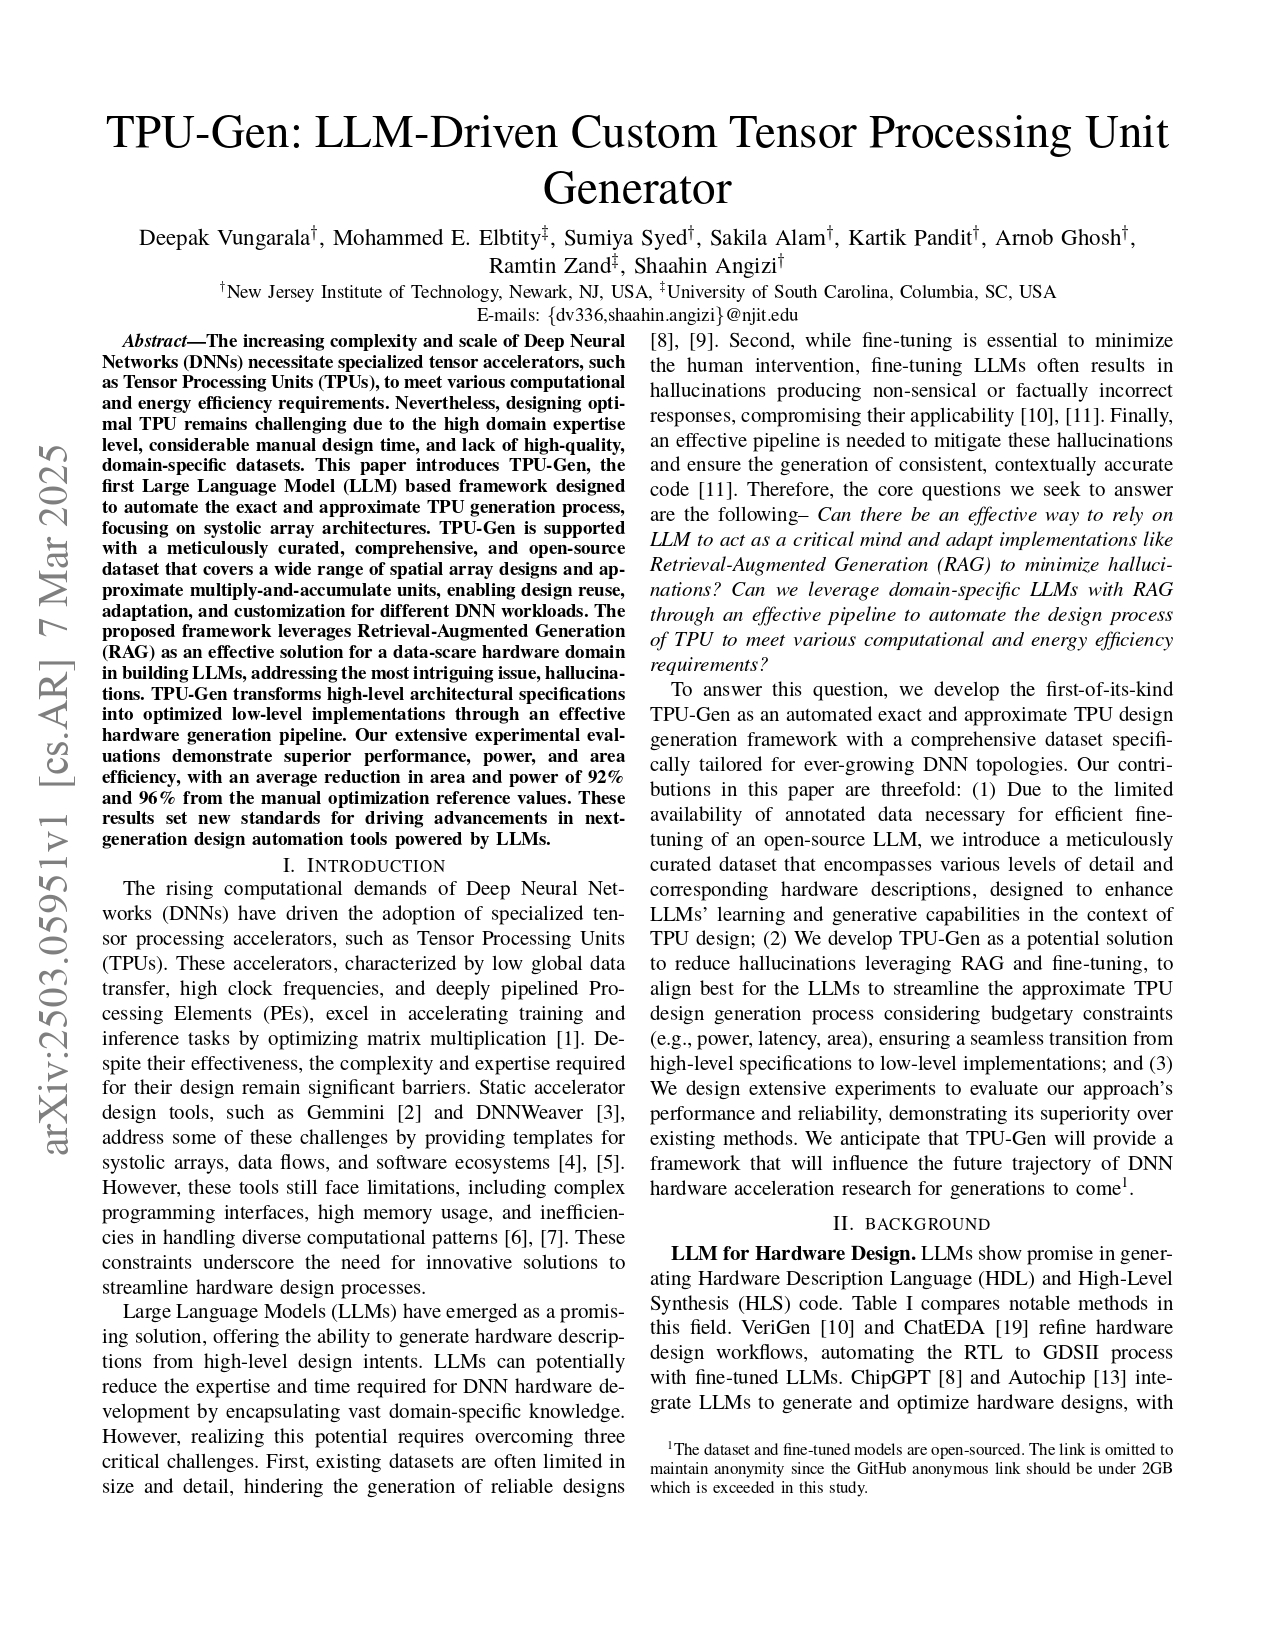
\includegraphics[width=0.9\linewidth, height=3.5cm, keepaspectratio, trim=0 400 0 0, clip]{images/LLMgen_page-0001.jpg}
}
};

\node[
  anchor=north west,
  fill=black!70,
  text=white,
  font=\scriptsize,
  inner sep=2pt
] at (img.north west) {TPU-Gen};

\node[
  anchor=south east,
  fill=black!70,
  text=white,
  font=\scriptsize,
  inner sep=2pt
] at (img.south east) {\cite{vungarala2025}};



\end{tikzpicture}

\vspace{0.4cm}


\begin{tikzpicture}
\node[inner sep=0] (img) {
  \fbox{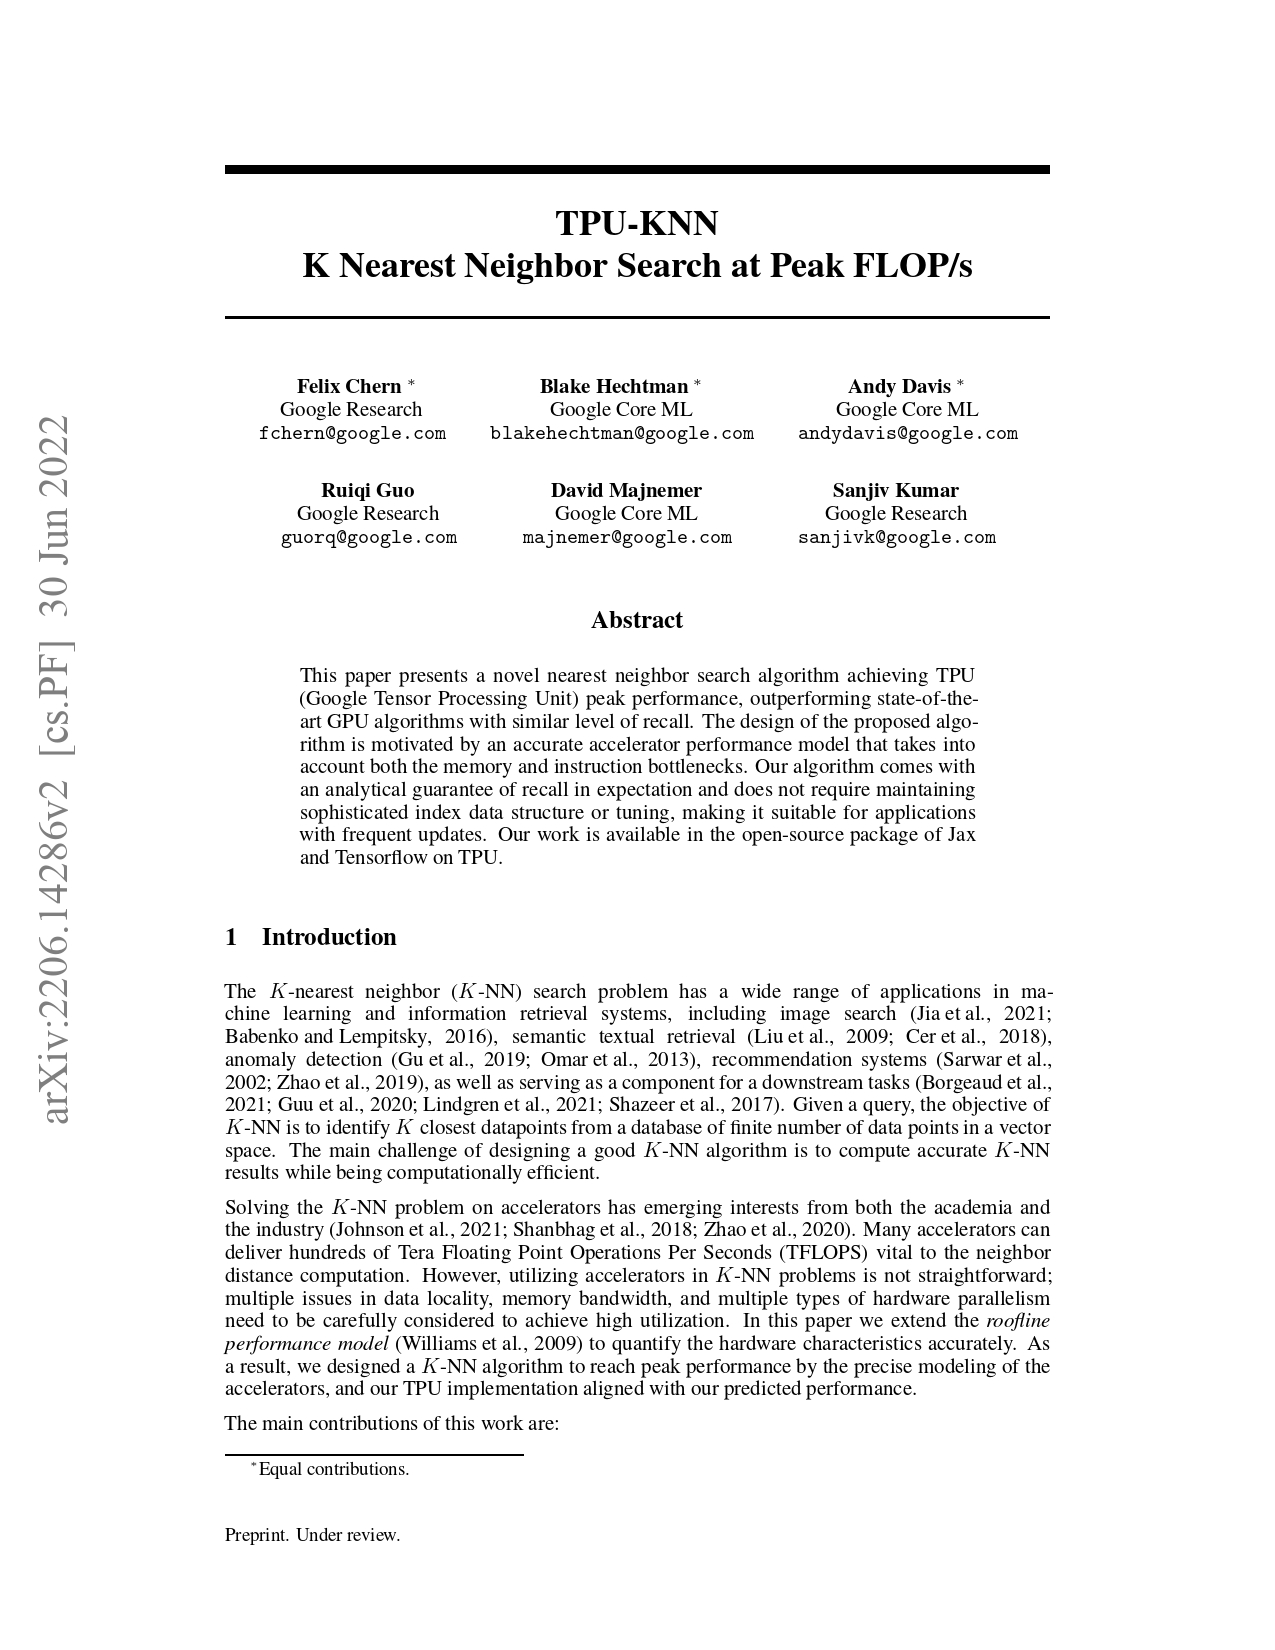
\includegraphics[width=0.9\linewidth, height=3.5cm, keepaspectratio, trim=0 400 0 0, clip]{images/TPUknn_page-0001.jpg}
}
};

\node[
  anchor=north west,
  fill=black!70,
  text=white,
  font=\scriptsize,
  inner sep=2pt
] at (img.north west) {TPU-KNN};

\node[
  anchor=south east,
  fill=black!70,
  text=white,
  font=\scriptsize,
  inner sep=2pt
] at (img.south east) {\cite{chern2022}};


\end{tikzpicture}

\end{columns}

\end{frame}

\section{Conclusão}
\begin{frame}{Conclusão}
  \begin{itemize}
    \item CPUs e GPUs não conseguiam
    atender a demanda de inferência em tempo real dos datacenters do Google

    \item Solução: \textbf{especialização radical} (abandonar cache, branch
    prediction e execução fora de ordem em favor de uma systolic array)

    \item Resultado: \textbf{15×–30× mais rápido} que contemporâneos,
    com \textbf{30×–80× melhor} eficiência energética

    \item \textbf{A TPU se tornou infraestrutura central da IA moderna}
  \end{itemize}

 \begin{block}{}
      \footnotesize\textit{``Minimalism is a virtue of\\domain-specific processors.''}\\
      \cite{jouppi2017tpu}
      
    \end{block}

\end{frame}

% ===== REFERÊNCIAS =====
\section{Referências}

% ----------------- SLIDE 16: REFERÊNCIAS -----------------
\begin{frame}[allowframebreaks]{Referências}
\bibliography{referencias}
\end{frame}
\begin{frame}{}
\centering
    \Huge Obrigado!
\end{frame}
% ----------------- FIM DO DOCUMENTO -----------------------------------------
\end{document}
